\section{System Architecture}
\label{sec:system-architecture}
We start our system architecture design from several key application requirements, mainly the users' point of view.

Imagine one wants to know his indoor location without painful process of looking at room number and compare it with a sophiscated map; the system should be able to detect his location and automatically generate the highlighted location with the display of a map. Meanwhile, {\em privacy} is an important issue that the localization should be computed locally and the user is able to control whether to share his location or not. Good {\em accuracy} and {\em responsiveness} are also required to ensure users' satisfaction of this system. 

In addition to the local display of location, interesting applications can be built upon the aggregation of users' information. We design one such application called Marauder's Map\footnote{http://harrypotter.wikia.com/wiki/Marauder's\_Map}, which could show the active location of other users. This requires the front-end and back-end design to provide accessibility of the aggregated information.


\begin{figure}
  \centering
  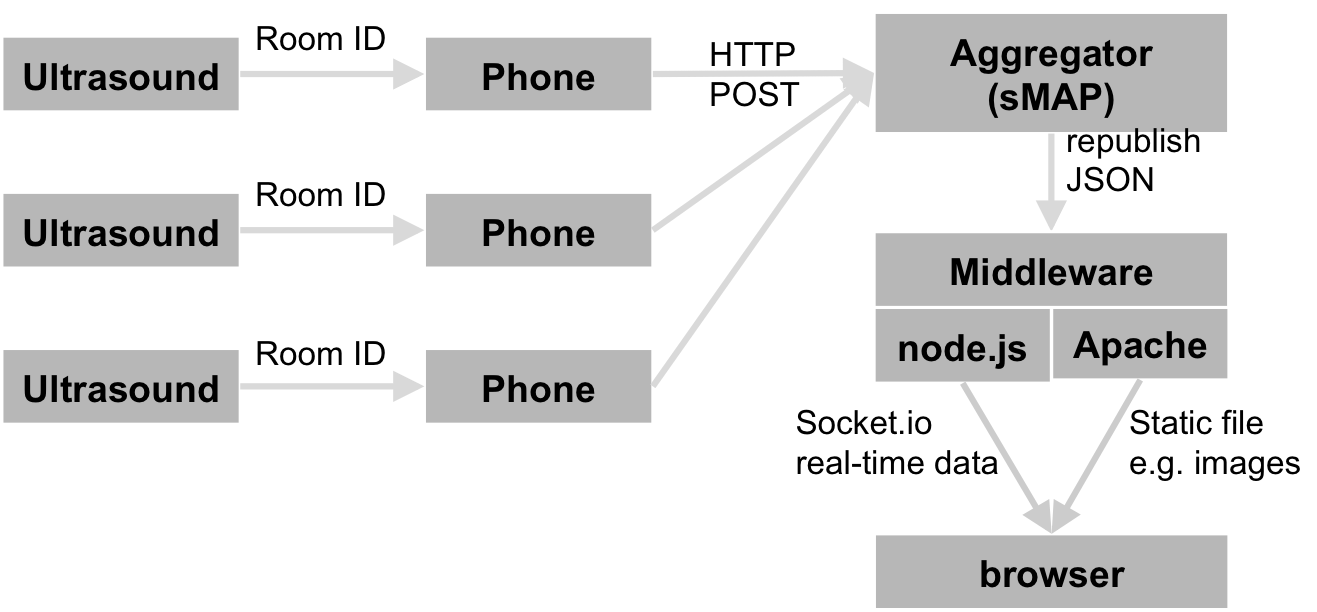
\includegraphics[width=\columnwidth]{sysarch.png}
  \caption{System Architecture for Marauder's Map}
  \label{fig:sysarch}
\end{figure}

Our system architecture is shown in Fig.\,\ref{fig:sysarch} where 
%% Master
%%% Local Variables: 
%%% mode: latex
%%% TeX-master: "ee149"
%%% End: 
